% Created 2014-05-11 日 20:08
\documentclass[11pt]{article}
\usepackage[utf8]{inputenc}
\usepackage[T1]{fontenc}
\usepackage{fixltx2e}
\usepackage{graphicx}
\usepackage{longtable}
\usepackage{float}
\usepackage{wrapfig}
\usepackage{soul}
\usepackage{textcomp}
\usepackage{marvosym}
\usepackage{wasysym}
\usepackage{latexsym}
\usepackage{amssymb}
\usepackage{hyperref}
\tolerance=1000
\providecommand{\alert}[1]{\textbf{#1}}

\title{sicp-chapter-1}
\author{yuen}
\date{\today}
\hypersetup{
  pdfkeywords={},
  pdfsubject={},
  pdfcreator={Emacs Org-mode version 7.9.3f}}

\begin{document}

\maketitle

\setcounter{tocdepth}{3}
\tableofcontents
\vspace*{1cm}
\section{Exercise 1.1.}
\label{sec-1}


  Below is a sequence of expressions. What is the result printed by the
  interpreter in response to each expression? Assume that the sequence is
  to be evaluated in the order in which it is presented.


\begin{verbatim}
10
(+ 5 3 4)
(- 9 1)
(/ 6 2)
(+ (* 2 4) (- 4 6))
(define a 3)
(define b (+ a 1))
(+ a b (* a b))
(= a b)
(if (and (> b a) (< b (* a b)))
    b
    a)
(cond ((= a 4) 6)
      ((= b 4) (+ 6 7 a))
      (else 25))
(+ 2 (if (> b a) b a))
(* (cond ((> a b) a)
         ((< a b) b)
         (else -1))
   (+ a 1))
\end{verbatim}


\begin{verbatim}
10
12
8
3
6
19
#f
4
16
6
16
\end{verbatim}
\section{Exercise 1.2.}
\label{sec-2}


  Translate the following expression into prefix form

\begin{equation}
\frac{5 + 4 + (2 - (3 - (6 + \frac{4}{5})))}{3 (6 - 2) (2 - 7)}
\end{equation}
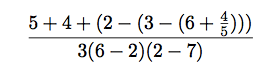
\includegraphics[width=.9\linewidth]{exercise-1.2.png}

\begin{verbatim}
(/ (+ 5 4 (- 2 (- 3 (+ 6 (/ 4 5))))) (* 3 (- 6 2) (- 2 7)))
\end{verbatim}

\begin{verbatim}
 -37/150
\end{verbatim}
\section{Exercise 1.3.}
\label{sec-3}


  Define a procedure that takes three numbers as arguments and returns the sum
  of the squares of the two larger numbers.


\begin{verbatim}
(define (bigger x y)
  (if (> x y) x y))

(define (smaller x y)
  (if (< x y) x y))

(define (bigger-sum a b c)
  (+ (sqr (bigger a b)) (sqr (bigger (smaller a b) c))))

(bigger-sum 1 2 3)
\end{verbatim}

\begin{verbatim}
 13
\end{verbatim}
\section{Exercise 1.4.}
\label{sec-4}


  Observe that our model of evaluation allows for combinations whose operators
  are compound expressions. Use this observation to describe the behavior of the
  following procedure:


\begin{verbatim}
(define (a-plus-abs-b a b)
  ((if (> b 0) + -) a b))

(a-plus-abs-b 1 1)
(a-plus-abs-b 1 -1)
\end{verbatim}

\begin{verbatim}
 2
 2
\end{verbatim}

  定义了一个函数 a-plus-abs-b,有两个参数 a b


\begin{verbatim}
(if (> b 0) + -)
\end{verbatim}

  如果 b 大于 0,那么返回 +,否则返回 -

  这里把操作符做为函数的返回值

  (op a b)
\section{Exercise 1.5.}
\label{sec-5}


  Ben Bitdiddle has invented a test to determine whether the interpreter he is
  faced with is using applicative-order evaluation or normal-order evaluation.
  He defines the following two procedures:


\begin{verbatim}
(define (p) (p))

(define (test x y)
  (if (= x 0)
      0
      y))
\end{verbatim}

Then he evaluates the expression


\begin{verbatim}
(test 0 (p))
\end{verbatim}

  What behavior will Ben observe with an interpreter that uses applicative-order
evaluation? What behavior will he observe with an interpreter that uses
normal-order evaluation? Explain your answer. (Assume that the evaluation rule
for the special form if is the same whether the interpreter is using normal or
applicative order: The predicate expression is evaluated first, and the result
determines whether to evaluate the consequent or the alternative expression.)

  applicative-order: 会在参数传递前进行表达式的执行,即: (test 0 (p))

  此时会先分别对表达式 0,(p) 分别求值,表达式 (p) 展开求值进入死循环

  normal-order: 会在用到参数时才进行求值,先将 0 和 (p) 带入 (test x y)

  此时判断 (if (= x 0) 0 (p)) 先执行 (= x 0) 即: (= 0 0),直接返回 0 并不再执行(p)
\section{Exercise 1.6.}
\label{sec-6}


  Alyssa P. Hacker doesn't see why if needs to be provided as a special form.
  ``Why can't I just define it as an ordinary procedure in terms of cond?''
  she asks. Alyssa's friend Eva Lu Ator claims this can indeed be done,
  and she defines a new version of if:


\begin{verbatim}
(define (new-if predicate then-clause else-clause)
  (cond (predicate then-clause)
        (else else-clause)))

; Eva demonstrates the program for Alyssa:

(new-if (= 2 3) 0 5)

(new-if (= 1 1) 0 5)
\end{verbatim}

\begin{verbatim}
 5
 0
\end{verbatim}

Delighted, Alyssa uses new-if to rewrite the square-root program:


\begin{verbatim}
(define (sqrt-iter guess x)
  (new-if (good-enough? guess x)
          guess
          (sqrt-iter (improve guess x)
                     x)))
\end{verbatim}

What happens when Alyssa attempts to use this to compute square roots? Explain.

这里的 new-if 是一个普通的函数,在函数调用时会先对其参数进行求值,

这里 new-if 的两个参数分别是函数调用 (goo-enough) 和 (sqrt-iter),对两个分别进行
求值计算就导致陷入了 (sqrt-iter) 的无限循环内

书上有写:

(if <predicate> <consequent> <alternative>) 的求值顺序是从 <predicate> 开始,

如果 <predicate> 得到真值,解释器会去求值 <consequent> 并返回其值,

否则它就去求值 <alternative> 并返回其值


\begin{verbatim}

(if #t (display "hello") (display "world"))
\end{verbatim}

\begin{verbatim}
 hello
\end{verbatim}



\begin{verbatim}

(define (new-if predicate then-clause else-clause)
  (cond (predicate then-clause)
        (else else-clause)))

(new-if #t (display "hello") (display "world"))
\end{verbatim}

\begin{verbatim}
 helloworld
\end{verbatim}


牛顿法求平方根的算法:


\begin{verbatim}
(define (abs x)
  (if (< x 0) (- 0 x) x))

(define (square x)
  (* x x))

(define (good-enough? guess x)
  (display (format "~a\n" guess))
  (< (abs (- (square guess) x)) 0.0001))

(define (improve guess x)
  (/ (+ guess (/ x guess)) 2))

(define (sqrt-iter guess x)
  (if (good-enough? guess x) guess
      (sqrt-iter (improve guess x) x)))

(define (sqrt x)
  (sqrt-iter 1.0 x))

(sqrt 9)

(sqrt 0.0000000000000000000009)
\end{verbatim}


\begin{verbatim}
1.0
5.0
3.4
3.023529411764706
3.00009155413138
3.000000001396984
3.000000001396984

1.0
0.5
0.25
0.125
0.0625
0.03125
0.015625
0.0078125
0.0078125
\end{verbatim}
\section{Exercise 1.7.}
\label{sec-7}


  The good-enough? test used in computing square roots will not be very
  effective for finding the square roots of very small numbers. Also,
  in real computers, arithmetic operations are almost always performed with
  limited precision. This makes our test inadequate for very large numbers.
  Explain these statements, with examples showing how the test fails for small
  and large numbers. An alternative strategy for implementing good-enough?
  is to watch how guess changes from one iteration to the next and to stop when
  the change is a very small fraction of the guess. Design a square-root
  procedure that uses this kind of end test.
  Does this work better for small and large numbers?

  针对非常小的数字,我们可以使用优化 good-enough 函数来解决


\begin{verbatim}
(define (abs x)
  (if (< x 0) (- 0 x) x))

(define (square x)
  (* x x))

(define (good-enough? old-guess new-guess)
  (display (format "~a\n" old-guess))
  (< (/ (abs (- new-guess old-guess)) old-guess) 0.0001))

(define (improve guess x)
  (/ (+ guess (/ x guess)) 2))

(define (sqrt-iter guess x)
  (let ((new-guess (improve guess x)))
    (if (good-enough? guess new-guess) guess
        (sqrt-iter new-guess x))))

(define (sqrt x)
  (sqrt-iter 1.0 x))

(sqrt 0.0000000000000000000009)
\end{verbatim}


\begin{verbatim}
1.0
0.5
0.25
0.125
0.0625
0.03125
0.015625
0.0078125
0.00390625
0.001953125
0.0009765625000000002
0.0004882812500000005
0.0002441406250000012
0.00012207031250000244
6.10351562500049e-05
3.0517578125009826e-05
1.5258789062519658e-05
7.629394531289321e-06
3.814697265703643e-06
1.9073486329697864e-06
9.536743167208228e-07
4.768371588322706e-07
2.384185803598537e-07
1.1920929206736365e-07
5.960464980855534e-08
2.9802332454024236e-08
1.4901181326501416e-08
7.450620862198706e-09
3.725370828750545e-09
1.8628062077192604e-09
9.316446748819594e-10
4.663053542092095e-10
2.341177099868953e-10
1.1898096502957087e-10
6.327260009878856e-11
3.8748383309721934e-11
3.098757940327563e-11
3.001573716141363e-11
3.000000412547338e-11
3.000000412547338e-11
\end{verbatim}
\section{Exercise 1.8.}
\label{sec-8}


  Newton's method for cube roots is based on the fact that if y is an
  approximation to the cube root of x, then a better approximation is
  given by the value

\begin{equation}
\frac{x/y^2 + 2y}{3}
\end{equation}

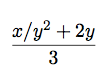
\includegraphics[width=.9\linewidth]{exercise-1.8.png}

  Use this formula to implement a cube-root procedure analogous to the
  square-root procedure.

  (In section 1.3.4 we will see how to implement
  Newton's method in general as an abstraction of these square-root and
  cube-root procedures.)

算法过程与开平方类似,我们只需要修改 `improve` 函数就可以:


\begin{verbatim}
(define (abs x)
  (if (< x 0) (- 0 x) x))

(define (square x)
  (* x x))

(define (good-enough? old-guess new-guess)
  (display (format "~a\n" old-guess))
  (< (/ (abs (- new-guess old-guess)) old-guess) 0.0001))

(define (improve guess x)
  (/ (+ (* 2 guess) (/ x (* guess guess))) 3))

(define (cube-root-iter guess x)
  (let ((new-guess (improve guess x)))
    (if (good-enough? guess new-guess) guess
        (cube-root-iter new-guess x))))

(define (cube-root x)
  (cube-root-iter 1.0 x))

(cube-root 0.000000008)
\end{verbatim}


\begin{verbatim}
1.0
0.6666666693333334
0.44444445222222223
0.296296314981481
0.19753090702931686
0.13168733969659827
0.08779171357094338
0.05852815503580874
0.03901954848882324
0.026014783802133092
0.017347129492363524
0.011573614622429779
0.007735651222160343
0.005201663871345835
0.003566332162406482
0.0025872193951923263
0.0021231972308747436
0.0020070101831742913
0.002000024457002051
0.002000024457002051
\end{verbatim}
\section{Exercise 1.9.}
\label{sec-9}


  Each of the following two procedures defines a method for adding two positive
  integers in terms of the procedures inc, which increments its argument by 1,
  and dec, which decrements its argument by 1.


\begin{verbatim}
(define (+ a b)
  (if (= a 0)
      b
      (inc (+ (dec a) b))))

(define (+ a b)
  (if (= a 0)
      b
      (+ (dec a) (inc b))))
\end{verbatim}

  Using the substitution model, illustrate the process generated by each
  procedure in evaluating (+ 4 5). Are these processes iterative or recursive?

  通过下面的例子我们也可以很容易看出来:第一个是递归的,第二个是迭代的


\begin{verbatim}
(define (inc x)
  (display (format "inc ~a\n" x))
  (+ x 1))

(define (dec x)
  (display (format "dec ~a\n" x))
  (- x 1))

(define (plus a b)
  (display (format "plus ~a ~a\n" a b))

  (if (= a 0)
      b
      (inc (plus (dec a) b))))

(plus 4 5)
\end{verbatim}



\begin{verbatim}
(define (inc x)
  (display (format "inc ~a\n" x))
  (+ x 1))

(define (dec x)
  (display (format "dec ~a\n" x))
  (- x 1))


(define (plus a b)
  (display (format "plus ~a ~a\n" a b))

  (if (= a 0)
      b
      (plus (dec a) (inc b))))

(plus 4 5)
\end{verbatim}
\section{Exercise 1.10.}
\label{sec-10}


  The following procedure computes a mathematical function called Ackermann's
  function.


\begin{verbatim}
(define (A x y)
  (cond ((= y 0) 0)
        ((= x 0) (* 2 y))
        ((= y 1) 2)
        (else (A (- x 1)
                 (A x (- y 1))))))
\end{verbatim}

What are the values of the following expressions?


\begin{verbatim}
(A 1 10)

(A 2 4)

(A 3 3)
\end{verbatim}

Consider the following procedures, where A is the procedure defined above:


\begin{verbatim}
(define (f n) (A 0 n))

(define (g n) (A 1 n))

(define (h n) (A 2 n))

(define (k n) (* 5 n n))
\end{verbatim}

Give concise mathematical definitions for the functions computed by the
procedures f, g, and h for positive integer values of n. For example, (k n)
computes 5n$^2$.



\begin{verbatim}
(define (A x y)
  (cond ((= y 0) 0)
        ((= x 0) (* 2 y))
        ((= y 1) 2)
        (else (A (- x 1)
                 (A x (- y 1))))))

(A 1 10)

(A 2 4)

(A 3 3)
\end{verbatim}



\begin{verbatim}
(define (A x y)
  (cond ((= y 0) 0)
        ((= x 0) (* 2 y))
        ((= y 1) 2)
        (else (A (- x 1)
                 (A x (- y 1))))))

(define (f n) (A 0 n))

(define (g n) (A 1 n))

(define (h n) (A 2 n))

(display "(f n)\n")
(for ([i 10])
  (display (format "~a: ~a\n" i (f i))))


(display "(g n)\n")
(for ([i 10])
  (display (format "~a: ~a\n" i (g i))))

(display "(h n)\n")
(for ([i 5])
  (display (format "~a: ~a\n" i (h i))))
\end{verbatim}

我们可以通过列表看出:

(f n) = 2n

(g n) = 2$^n$

(h n) = 2$^2$$^2$\ldots{}{n\}
\section{Exercise 1.11.}
\label{sec-11}


  A function f is defined by the rule that

  f(n) = n if n<3 and
  f(n) = f(n - 1) + 2f(n - 2) + 3f(n - 3) if n> 3.

  Write a procedure that computes f by means of a recursive process.

  Write a procedure that computes f by means of an iterative process.


  递归的版本比较好写,我们先看下:


\begin{verbatim}
(define (rec-f n)
  (if (< n 3)
      n
      (+ (rec-f (- n 1))
         (* 2 (rec-f (- n 2)))
         (* 3 (rec-f (- n 3))))))

(rec-f 0)
(rec-f 1)
(rec-f 2)
(rec-f 3)
(rec-f 4)
\end{verbatim}


迭代和递归相比,我们需要自己来传递上一次计算的结果



\begin{verbatim}
(define (iter-f-iter a b c i n)
  (display (format "a=~a, b=~a, c=~a, i=~a\n" a b c i))
  (if (= i n)
      c
      (iter-f-iter (+ a (* 2 b) (* 3 c))
                   a
                   b
                   (+ i 1)
                   n)))

(define (iter-f n)
  (iter-f-iter 2 1 0 0 n))

(iter-f 4)
\end{verbatim}
\section{Exercise 1.12.}
\label{sec-12}


  The following pattern of numbers is called Pascal's triangle.


          1
        1   1
      1   2   1
    1   3   3   1
  1   4   6   4   1

  The numbers at the edge of the triangle are all 1, and each number inside
  the triangle is the sum of the two numbers above it.35 Write a procedure that
  computes elements of Pascal's triangle by means of a recursive process.



\begin{verbatim}

(define (pascal row col)
  (cond ((> col row) (error "row less then cow"))
        ((or (= col 0) (= row col)) 1)
        (else (+ (pascal (- row 1) (- col 1)) (pascal (- row 1) col)))))

(pascal 1 1)

(pascal 3 2)
\end{verbatim}
\section{Exercise 1.13.}
\label{sec-13}


 Prove that Fib(n) is the closest integer to φ$^n$ / √5, where φ = (1 + √5) / 2.
 Hint: Let ψ = (1 - √5) / 2. Use induction and the definition of the Fibonacci
 numbers (see section 1.2.2) to prove that

 Fib(n) = (φ$^n$ - ψ$^n$) / √5.


 Fib(n) = (((1 + √5) / 2)$^n$ - ((1 - √5) / 2)$^n$) / √5.

 我们先把这个式子写成代码看一下结果:



\begin{verbatim}

(define (fib n)
  (cond ((< n 0) (error "n is less then 0"))
        ((= n 0) 0)
        ((= n 1) 1)
        ((= n 2) 1)
        (else (+ (fib (- n 1)) (fib (- n 2))))))

(displayln (fib 6))

(define (fib n)
  ( / (- (expt (/ (+ 1 (sqrt 5)) 2) n)
         (expt (/ (- 1 (sqrt 5)) 2) n))
      (sqrt 5)))

(displayln (fib 6))
\end{verbatim}


证明:

 Fib(1) = (((1 + √5) / 2) - ((1 - √5) / 2)) / √5 = 1

 \ldots{}

 Fib(n) = (((1 + √5) / 2)$^n$ - ((1 - √5) / 2)$^n$) / √5 = (φ$^n$ - ψ$^n$) / √5

 Fib(n + 1) = (φ^(n+1) - ψ^(n+1)) / √5 = (φφ$^n$ - ψψ$^n$) / √5 =
              (((1 + √5) / 2)φ$^n$ - ((1 - √5) / 2)ψ$^n$) / √5 =
              (1/2)(Fib(n) + φ$^n$ + ψ$^n$)

 Fib(n + 2) = (3/2)(Fib(n) + φ$^n$ + ψ$^n$) = Fib(n) + Fib(n + 1)

 符合Fib的定义
\section{Exercise 1.14.}
\label{sec-14}


  Draw the tree illustrating the process generated by the count-change procedure
  of section 1.2.2 in making change for 11 cents. What are the orders of growth
  of the space and number of steps used by this process as the amount to be
  changed increases?



\begin{verbatim}
(require trace)

(define (first-denomination kinds-of-coins)
  (cond ((= kinds-of-coins 1) 1)
        ((= kinds-of-coins 2) 5)
        ((= kinds-of-coins 3) 10)
        ((= kinds-of-coins 4) 25)
        ((= kinds-of-coins 5) 50)))


(define (cc amount kinds-of-coins)
  (cond ((= amount 0 ) 1)
        ((or (< amount 0) (= kinds-of-coins 0)) 0)
        (else (+ (cc amount (- kinds-of-coins 1))
                 (cc (- amount (first-denomination kinds-of-coins))
                     kinds-of-coins)))))

(define (count-change amount)
  (cc amount 5))


(displayln (count-change 11))
\end{verbatim}

racket下,在代码里加上=(require trace)=就可以对函数调用进行跟踪,从而得到递归调用堆栈
\section{Exercise 1.15.}
\label{sec-15}

  The sine of an angle (specified in radians) can be computed by making use of
  the approximation sin x  x if x is sufficiently small, and the trigonometric
  identity

\begin{equation}
\sin x = 3\sin \frac{x}{3} - 4\sin^3\frac{x}{3}
\end{equation}

  to reduce the size of the argument of sin. (For purposes of this exercise an
  angle is considered ``sufficiently small'' if its magnitude is not greater than
  0.1 radians.) These ideas are incorporated in the following procedures:


\begin{verbatim}
(define (cube x) (* x x x))
(define (p x) (- (* 3 x) (* 4 (cube x))))
(define (sine angle)
   (if (not (> (abs angle) 0.1))
       angle
       (p (sine (/ angle 3.0)))))
\end{verbatim}

a.  How many times is the procedure p applied when (sine 12.15) is evaluated?

b.  What is the order of growth in space and number of steps
(as a function of a) used by the process generated by the sine procedure when
(sine a) is evaluated?

\end{document}
